\documentclass[a4paper,11pt]{article}

% Packages
\usepackage[utf8]{inputenc}
\usepackage[T1]{fontenc}
\usepackage{lmodern}           % Latin Modern fonts (vectorielles, pas bitmap)
\usepackage{microtype}         % Améliore le rendu typographique
\usepackage{babel}
\usepackage{geometry}
\usepackage{xcolor}
\usepackage{enumitem}
\usepackage{titlesec}
\usepackage{tcolorbox}
\usepackage{graphicx}
\usepackage{fancyhdr}
\usepackage{tabularx}
\usepackage{booktabs}
\usepackage{multicol}
\usepackage{tikz}
\usepackage{amsmath}
\usepackage{amssymb}
\usepackage{hyperref}
\usepackage{natbib}

% Définition des couleurs violet/lavande
\definecolor{mainpurple}{RGB}{106, 90, 205}      % Slate Blue
\definecolor{lightlavender}{RGB}{230, 230, 250}  % Lavender
\definecolor{deeppurple}{RGB}{75, 0, 130}        % Indigo
\definecolor{softpurple}{RGB}{147, 112, 219}     % Medium Purple
\definecolor{palelavender}{RGB}{245, 240, 255}   % Très pâle

% Configuration de la page
\geometry{
    top=2.5cm,
    bottom=2.5cm,
    left=2.5cm,
    right=2.5cm,
    headheight=22pt
}

% En-têtes et patins de page
\pagestyle{fancy}
\fancyhf{}
\fancyhead[L]{\color{mainpurple}\small\leftmark}
\fancyfoot[C]{\color{mainpurple}\thepage}
\renewcommand{\headrulewidth}{0.5pt}
\renewcommand{\footrulewidth}{0.5pt}
\renewcommand{\headrule}{\hbox to\headwidth{\color{mainpurple}\leaders\hrule height \headrulewidth\hfill}}
\renewcommand{\footrule}{\hbox to\headwidth{\color{mainpurple}\leaders\hrule height \footrulewidth\hfill}}

% Configuration des titres
\titleformat{\section}
  {\LARGE\bfseries\color{deeppurple}}
  {\thesection}{1em}{}
  [\titlerule]

\titleformat{\subsection}
  {\Large\bfseries\color{mainpurple}}
  {\thesubsection}{1em}{}

\titleformat{\subsubsection}
  {\large\bfseries\color{softpurple}}
  {\thesubsubsection}{1em}{}

% Environnements pour les boîtes
\newtcolorbox{infobox}{
    colback=lightlavender,
    colframe=mainpurple,
    boxrule=1pt,
    arc=3mm,
    left=10pt,
    right=10pt,
    top=10pt,
    bottom=10pt
}

\newtcolorbox{tipbox}{
    colback=palelavender,
    colframe=softpurple,
    boxrule=1pt,
    arc=3mm,
    left=10pt,
    right=10pt,
    top=10pt,
    bottom=10pt,
    title={\textbf{$\triangleright$ Conseil pratique}}
}

\newtcolorbox{warningbox}{
    colback=lightlavender!50,
    colframe=deeppurple,
    boxrule=1.5pt,
    arc=3mm,
    left=10pt,
    right=10pt,
    top=10pt,
    bottom=10pt,
    title={\textbf{$\blacktriangledown$ Attention}}
}

\newtcolorbox{examplebox}{
    colback=palelavender,
    colframe=mainpurple,
    boxrule=1pt,
    arc=2mm,
    left=8pt,
    right=8pt,
    top=8pt,
    bottom=8pt,
    title={\textbf{$\star$ Exemple concret}}
}

% Configuration des liens
\hypersetup{
    colorlinks=true,
    linkcolor=deeppurple,
    filecolor=mainpurple,
    urlcolor=softpurple,
}

% Document
\begin{document}

% Page de titre
\begin{titlepage}
    \centering
    \vspace*{2cm}

    {\Huge\bfseries\color{deeppurple} Guide Complet\par}
    \vspace{0.3cm}
    {\Huge\bfseries\color{mainpurple} d'entraînement\par}
    \vspace{0.3cm}
    {\Huge\bfseries\color{softpurple} à l'aim\par}

    \vspace{1.5cm}

    \begin{tcolorbox}[
        colback=lightlavender,
        colframe=mainpurple,
        width=0.85\textwidth,
        arc=5mm,
        boxrule=2pt
    ]
    \centering
    {\Large\color{deeppurple} De la théorie à la pratique :\par}
    \vspace{0.4cm}
    {\large Maîtrisez tous les aspects du gaming FPS\par}
    \vspace{0.2cm}
    {\large pour devenir un joueur d'élite\par}
    \end{tcolorbox}

    \vspace{1cm}

    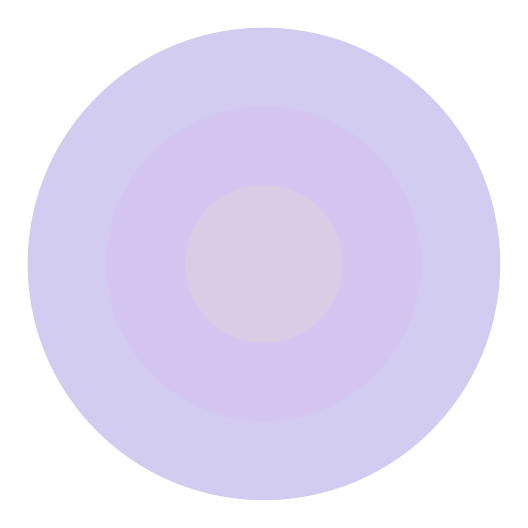
\begin{tikzpicture}
        \fill[mainpurple!30] (0,0) circle (3cm);
        \fill[softpurple!40] (0,0) circle (2cm);
        \fill[deeppurple!20] (0,0) circle (1cm);
    \end{tikzpicture}

    \vfill

    {\large\textbf{\color{mainpurple} Par : a1ka}\par}

    \vspace{0.8cm}

    {\large\color{softpurple}\today\par}
\end{titlepage}

% Table des matières
\tableofcontents
\newpage

\section{Introduction}

La visée, ou "aim" en anglais, est l'une des compétences fondamentales dans les jeux de tir à la première personne (FPS). Contrairement à ce que l'on pourrait penser, elle ne se résume pas simplement à la capacité de pointer sa souris vers un ennemi. Il s'agit d'un ensemble complexe de compétences motrices, cognitives et stratégiques qui, une fois maîtrisées, peuvent faire toute la différence entre la victoire et la défaite.

\begin{infobox}
Ce guide a pour objectif de démystifier \textbf{tous les aspects} du FPS compétitif : de la compréhension théorique de l'aim jusqu'au choix du matériel, en passant par l'optimisation de vos paramètres et la préservation de votre santé. Nous aborderons chaque élément de manière pédagogique et accessible.
\end{infobox}

\subsection{À qui s'adresse ce guide ?}

Ce guide est conçu pour :
\begin{itemize}
    \item \textbf{Les débutants} qui souhaitent comprendre les fondamentaux du FPS compétitif
    \item \textbf{Les joueurs intermédiaires} cherchant à optimiser leur progression
    \item \textbf{Les joueurs avancés} voulant affiner leurs connaissances et corriger de mauvaises habitudes
    \item \textbf{Toute personne} intéressée par la compréhension scientifique et méthodologique de la performance en gaming
\end{itemize}

\subsection{Structure du guide}

Ce guide est divisé en plusieurs parties complémentaires :
\begin{enumerate}
    \item \textbf{Théorie de l'aim} : Comprendre les mécanismes de l'aim
    \item \textbf{Matériel et équipement} : Choisir le bon setup pour performer
    \item \textbf{Paramètres et configuration} : Optimiser sensibilité, vidéo et périphériques
    \item \textbf{Méthodologie d'entraînement} : Structurer sa progression
    \item \textbf{Santé et ergonomie} : Jouer durablement sans se blesser
    \item \textbf{Aspects mentaux} : Développer la bonne mentalité
\end{enumerate}

\newpage

\section{Comprendre l'aim : anatomie d'une compétence complexe}

\subsection{Les deux piliers de l'aim}

L'aim se décompose en deux catégories distinctes mais complémentaires : l'aim passive et l'aim active. Cette distinction est fondamentale pour comprendre comment s'entraîner efficacement.

\subsubsection{L'aim passive : la fondation invisible}

L'aim passive représente l'ensemble des compétences qui vous permettent de \textbf{minimiser le besoin d'ajustement} de votre aim. 

C'est la partie "préventive" de votre aim. Elle comprend :
\begin{itemize}
    \item \textbf{Le crosshair placement :} Il s'agit de la position de votre viseur à tout moment du jeu. Un bon placement signifie que votre aim est déjà approximativement sur la cible avant même que l'ennemi n'apparaisse. Vous anticipez les angles, les hauteurs de tête, et les positions probables des adversaires.

    \item \textbf{Les déplacements (counter-strafe) :} Dans les FPS tactiques comme Counter-Strike ou Valorant, votre précision est grandement affectée par vos mouvements. Le counter-strafe est la technique qui consiste à appuyer brièvement sur la touche opposée à votre direction de déplacement pour vous arrêter instantanément et retrouver votre précision maximale.

    \item \textbf{Le jiggle-peeking et la décale:} Le jiggle-peeking est une technique de déplacement permettent de collecter de l'information ou de provoquer un tir adverse tout en minimisant votre exposition. Ensuite, quand vous avez obtenu l'information, vous pouvez décaler de manière \textit{ciblée} l'ennemi. Ces principes font partie intégrante de la gestion des duels.

    \item \textbf{Le positionnement :} Au-delà de l'aim pure, savoir où se placer sur la carte pour avoir l'avantage dans les duels est crucial. Un bon positionnement vous fera gagner énormément de duels, mais on l'abordera plus en détail plus tard.
\end{itemize}

\begin{infobox}
\textbf{Pourquoi l'aim passive est-elle cruciale ?}

Dans les jeux à temps de réaction court comme CS2 ou Valorant, un joueur avec une aim passive excellente tuera 70 à 80\% de ses adversaires sans jamais avoir à effectuer un ajustement significatif de sa aim. On parle ici de \textbf{TTK} (=time to kill) faible.

Son viseur est déjà sur la cible au moment où elle apparaît.
\medbreak 

Je vais volontairement rester flou ici, mais si on devait découper un duel :

\begin{itemize}
    \item Apparition de l'ennemi : le temps que ça monte au cerveau ~~~~    \textcolor{mainpurple}{150-350ms*}
    \item Ajustement : déplacer le viseur sur l'ennemi ~~~~~~~~~~~~~~~~~~~~~~~~~~\textcolor{mainpurple}{50-150ms*}
    \item Cliquer
\end{itemize}

Si t'es tout le temps déjà sur la cible au moment où elle apparait, pas besoin d'ajuster !
\bigbreak 

\textcolor{mainpurple}{* : basé sur des moyennes scientifiques}
\end{infobox}

\subsubsection{L'aim active : l'ajustement réactif}

L'aim active, à l'inverse, concerne votre capacité à \textbf{corriger et ajuster} votre aim en temps réel. C'est la partie "réactive" de votre aim. Elle englobe :

\begin{itemize}
    \item \textbf{Le flicking :} La capacité à déplacer rapidement et précisément votre viseur d'un point A vers un point B. C'est le mouvement explosif que vous effectuez lorsqu'un ennemi apparaît à un endroit inattendu.

    \item \textbf{Le tracking :} La capacité à suivre une cible en mouvement de manière fluide.

    \item \textbf{Le temps de réaction :} Le délai entre le moment où vous percevez une information visuelle (un ennemi qui apparaît) et le moment où vous initiez votre action (déplacer votre souris, cliquer).

    \item \textbf{Les micro-ajustements :} Ces petits mouvements presque imperceptibles qui vous permettent d'affiner votre aim au dernier moment avant de tirer.

    \item \textbf{Le target switching :} La capacité à enchaîner rapidement plusieurs cibles différentes (crucial pour les "sprays transfer", par exemple).
\end{itemize}

\begin{examplebox}
\textbf{Scénarios concret illustrant l'aim active :}

Vous tenez une ligne correctement, mais l'ennemi sort d'une autre : il faut flick.

Vous êtes en duel avec quelqu'un qui bouge bien, mais l'ennemi strafe correctement : il faut ajuster en permanence.

etc.
\end{examplebox}
Comme vous le voyez, c'est des situations qui ne reflètent pas tous les jeux. Il faudra choisir correctement le programme d'entraînement, pour optimiser les exercices afin de correspondre au mieux au jeu traité.


\subsection{L'interdépendance des deux composantes}

Il est essentiel de comprendre que ces deux aspects de l'aim ne sont pas indépendants. Même avec une aim passive parfaite, vous rencontrerez inévitablement des situations imprévisibles : un ennemi qui sort d'un angle inhabituel, un adversaire qui saute, un spray transfer nécessaire entre deux cibles, ou simplement une erreur de positionnement de votre part.

C'est précisément dans ces moments que l'aim active devient indispensable. Si vous n'êtes pas capable d'ajuster rapidement et précisément votre aim, même la meilleure aim passive du monde ne suffira pas. C'est pourquoi, même si l'aim passive est prioritaire, négliger complètement l'aim active serait une erreur stratégique.

\begin{tipbox}
\textbf{Ratio d'entraînement recommandé :}
\begin{itemize}
    \item Jeux tactiques (CS2, Valorant) : 70\% aim passive / 30\% aim active
    \item Jeux dynamiques (Apex, Overwatch) : 30\% aim passive / 70\% aim active
    \item Jeux hybrides (Call of Duty) : 50\% aim passive / 50\% aim active, à adapter...
\end{itemize}
\end{tipbox}

\newpage

\section{Le matériel : fondations de la performance}

Avant même de parler d'entraînement, il est crucial de comprendre l'impact du matériel sur vos performances. Un mauvais setup peut créer un plafond de verre qui limitera votre progression, peu importe vos efforts.

\subsection{La souris : votre outil de précision}

\subsubsection{Critères de choix essentiels}

\begin{itemize}
    \item \textbf{Le capteur :} Privilégiez les capteurs optiques modernes (PixArt PMW3360/3389, Hero, Focus+ - et plus récents). Évitez les capteurs laser qui souffrent d'accélération et de prédiction.

    \item \textbf{Le poids :} Question très personnelle, mais la tendance actuelle favorise les souris légères ($60-80$g) et très légères ($60$g). Plus la souris est légère, moins vous dépensez d'énergie pour la contrôler, mais cela peut aussi réduire le contrôle fin.

    \item \textbf{La forme (shape) :} Critère le plus important. La souris doit épouser naturellement votre main selon votre style de préhension :
    \begin{itemize}
        \item \textit{Palm grip} : Toute la main sur la souris (nécessite une souris plus grande)
        \item \textit{Claw grip} : Doigts arqués, paume en contact arrière (souris moyenne)
        \item \textit{Fingertip grip} : Seuls les doigts touchent (souris petite et légère)
    \end{itemize}

    \item \textbf{Le polling-rate :} 1000 Hz minimum pour le gaming compétitif. Certains joueurs préfèrent 500 Hz pour plus de consistance ; d'autres ont des capteurs 8000 Hz pour la précision. Faites selon le ressenti.

    \item \textbf{Les patins (skates) :} Influencent la glisse. Les patins en PTFE (téflon) sont les plus courants. Certains joueurs remplacent les patins d'origine par des versions aftermarket pour optimiser la glisse.
\end{itemize}

\begin{warningbox}
Ne tombez pas dans le piège du marketing ! Une souris à 150€ n'est pas forcément meilleure qu'une souris à 50€. Ce qui compte, c'est l'adéquation avec VOTRE main et VOTRE style de jeu. Testez avant d'acheter si possible.
\end{warningbox}

\subsubsection{Souris recommandées par catégorie}

\begin{table}[h]
\centering
\begin{tabularx}{\textwidth}{|l|X|l|}
\hline
\textbf{Catégorie} & \textbf{Modèles populaires} & \textbf{Prix} \\
\hline
Budget & Logitech G203, Razer Viper Mini & 20-40€ \\
\hline
Mid-range & Logitech G Pro X Superlight, Razer DeathAdder V3 & 60-100€ \\
\hline
Premium & Finalmouse, Logitech G Pro X 2 Superlight, WLMouse Beast X& 100-180€ \\
\hline
\end{tabularx}
\caption{Exemples de souris par gamme de prix}
\end{table}
Note : ces prix sont à titre indicatifs. 

Renseignez-vous bien sur les souris \textbf{avant d'acheter} (i.e : bug de molette sur les G Pro)

\subsection{Le tapis de souris : l'infrastructure négligée}

Le tapis de souris est souvent sous-estimé, alors qu'il a un impact majeur sur le contrôle et la consistance.

\subsubsection{Types de surface}

\begin{itemize}
    \item \textbf{Tissu (cloth) :} Offre plus de contrôle, meilleure friction. Idéal pour la précision. Nécessite un nettoyage régulier.
    \item \textbf{Hybride :} Compromis entre vitesse et contrôle. Souvent traité avec un revêtement spécial.
    \item \textbf{Dur (hard pad / glass pad) :} Très rapide, faible friction. Préféré pour le tracking rapide. Plus durable mais moins de contrôle.
\end{itemize}

\subsubsection{Taille du tapis}
Voici les tailles standards des tapis (faites selon vos besoins, évidemment) :
\begin{table}[h]
\centering
\begin{tabularx}{\textwidth}{|l|X|X|}
\hline
\textbf{Taille} & \textbf{Dimensions} & \textbf{Recommandé pour} \\
\hline
Medium & 30-35 cm × 25-30 cm & Sensibilité moyenne à haute \\
\hline
Large & 40-45 cm × 35-40 cm & Sensibilité basse (recommandé) \\
\hline
Extended & 80-100 cm × 30-40 cm & Setup complet (clavier inclus) \\
\hline
\end{tabularx}
\caption{Tailles de tapis selon la sensibilité}
\end{table}

\begin{tipbox}
Privilégiez toujours un tapis \textbf{plus grand} que ce que vous pensez nécessaire. Cela vous évitera de heurter les bords lors de mouvements amples et vous permettra d'ajuster votre sensibilité vers le bas si besoin.
\end{tipbox}

\subsection{L'écran : voir pour réagir}

L'écran est votre fenêtre sur le jeu. Ses caractéristiques influencent directement votre temps de réaction et votre confort visuel.

\subsubsection{Taux de rafraîchissement (Hz)}

\begin{itemize}
    \item \textbf{60 Hz :} Standard, mais insuffisant pour le gaming compétitif (latence de 16.7ms par frame)
    \item \textbf{144 Hz :} Minimum recommandé pour le FPS compétitif (6.9ms par frame)
    \item \textbf{240 Hz :} Standard actuel du haut niveau (4.2ms par frame)
    \item \textbf{360 Hz / 480 Hz :} Avantage marginal mais perceptible au très haut niveau
\end{itemize}

\begin{infobox}
\textbf{Le mythe du "l'œil humain ne voit que 60 FPS"}

C'est faux. L'œil humain ne fonctionne pas en "images par seconde". La différence entre 60 Hz et 144 Hz est immédiatement perceptible, et même la différence entre 144 Hz et 240 Hz est notable pour la plupart des joueurs. Au-delà, les gains deviennent effectivement marginaux.
\end{infobox}

\subsubsection{Temps de réponse (ms)}

Le temps que met un pixel à changer de couleur. Pour le gaming :
\begin{itemize}
    \item \textbf{< 1 ms (MPRT)} : Excellent, aucun ghosting visible
    \item \textbf{1-3 ms (GtG)} : Très bon pour le gaming compétitif
    \item \textbf{4-5 ms} : Acceptable, léger ghosting possible
    \item \textbf{> 5 ms} : À éviter pour le FPS compétitif
\end{itemize}

\subsubsection{Technologie de dalle}

\begin{table}[h]
\centering
\begin{tabularx}{\textwidth}{|l|X|X|}
\hline
\textbf{Type} & \textbf{Avantages} & \textbf{Inconvénients} \\
\hline
TN & Temps de réponse le plus rapide, prix abordable & Angles de vision limités, couleurs ternes \\
\hline
IPS & Excellentes couleurs, bons angles de vision & Temps de réponse légèrement supérieur \\
\hline
VA & Bon contraste, prix moyen & Ghosting possible, temps de réponse variable \\
\hline
OLED & Noir parfait, temps de réponse instantané & Prix élevé, risque de burn-in \\
\hline
\end{tabularx}
\caption{Comparaison des technologies de dalle}
\end{table}

\begin{tipbox}
Pour le FPS compétitif, les dalles \textbf{TN} ou \textbf{IPS rapides} (< 1ms) sont recommandées. Les technologies comme Fast IPS, Nano IPS ou TN moderne offrent le meilleur compromis performance/qualité.
\end{tipbox}

\subsubsection{Taille et résolution}

\begin{itemize}
    \item \textbf{24 pouces @ 1080p (Full HD)} : Standard du FPS compétitif. Tout le champ de vision est facilement perceptible sans mouvement de tête. Moins exigeant pour la carte graphique.

    \item \textbf{27 pouces @ 1440p (2K)} : Excellent compromis qualité/performance pour les joueurs qui souhaitent plus de détails et d'immersion.

    \item \textbf{27+ pouces @ 2160p (4K)} : Magnifique visuellement, mais très exigeant. Non recommandé pour le compétitif pur (difficulté à maintenir des FPS élevés).
\end{itemize}

\begin{warningbox}
En FPS compétitif, privilégiez toujours les \textbf{FPS élevés} (240+ FPS) plutôt que la résolution. Un écran 1080p @ 240 Hz avec 300 FPS sera toujours plus réactif qu'un 1440p @ 144 Hz avec 150 FPS.
\end{warningbox}

\subsection{Les périphériques secondaires}

\subsubsection{Le clavier}

Bien que moins crucial que la souris pour l'aim, le clavier influence votre mobilité et vos capacités de mouvement.

\begin{itemize}
    \item \textbf{Switches mécaniques recommandés :}
    \begin{itemize}
        \item \textit{Cherry MX Red / Speed Silver} : Linéaires, rapides, aucun feedback tactile
        \item \textit{Cherry MX Brown} : Léger bump tactile, bon compromis
        \item \textit{Cherry MX Black} : Plus lourds, plus de contrôle
    \end{itemize}
    
    Note : il existe des claviers à \textcolor{mainpurple}{switches optique} qui sont généralement mieux et plus réactifs que les mécaniques grâce à leur technologie (Wooting, par exemple). Je ne recommanderai pas forcément si vous n'êtes pas déjà à niveau quasi-professionnel. Mais, pour la culture, ça existe !

    \item \textbf{Format :} Les formats TKL (TenKeyLess) ou 60\% sont privilégiés pour libérer de l'espace pour la souris.

    \item \textbf{Polling rate :} 1000 Hz pour une réactivité optimale.

\end{itemize}

\subsubsection{Le casque / Les écouteurs}

Le son spatial est crucial dans les FPS compétitifs pour la détection des ennemis.

\begin{itemize}
    \item \textbf{Privilégiez le stéréo} : Le "surround virtuel 7.1" est souvent un gadget marketing. Un bon casque stéréo avec des drivers de qualité offrira une meilleure spatialisation.

    \item \textbf{Type :}
    \begin{itemize}
        \item \textit{Fermé} : Isole des bruits extérieurs, meilleure immersion
        \item \textit{Ouvert} : Son plus naturel, meilleure spatialisation, mais laisse passer le bruit ambiant
    \end{itemize}

    \item \textbf{Microphone :} Clair, compréhensible, ... n'importe quoi fera l'affaire tant que ça grésille pas et que c'est bien réglé !
\end{itemize}


\newpage
\section{Mémoire musculaire et changement de sensibilité}

\subsection{Le mythe de la "muscle memory"}

Le terme \textit{muscle memory} est souvent utilisé en aim training, mais il est ambigu et trompeur. Il laisse penser que viser consiste à mémoriser précisément des mouvements, alors qu’il s’agit en réalité de développer des compétences spécifiques : contrôle de la souris, coordination œil-main, réactivité, lecture des trajectoires et fluidité. L’aim training vise donc à améliorer ces capacités, et non à enregistrer toutes les amplitudes de mouvement possibles.

\subsection{Pourquoi garder la même sensibilité semble rassurant}

La familiarité avec une sensibilité donnée est réelle, mais principalement à court terme. En jouant longtemps avec la même sensibilité, on développe une perception stable du lien entre mouvement physique et rotation en jeu, ainsi qu’une habitude dans la répartition de l’effort entre doigts, poignet, coude et épaule (wrist aim vs arm aim). 

Cependant, il est impossible de mémoriser parfaitement des distances de mouvement : le tapis de souris, l’humidité, l’usure, les micro-particules ou encore la position du bras varient constamment. La sensation change donc toujours légèrement.

\subsection{Changer de sensibilité : impact réel}

Changer de sensibilité ne ruine pas l’aim. Cela nécessite simplement une phase de réadaptation, plus ou moins importante selon l’ampleur du changement. Les modifications drastiques peuvent forcer un rééquilibrage dans l’utilisation des segments du bras, ce qui demande davantage d’ajustement.

Il est toutefois possible de développer sa capacité d’adaptation. De nombreux joueurs changent régulièrement de sensibilité — certains utilisent même des randomizers — sans pénalité notable à long terme. Modifier sa sensibilité peut même aider à dépasser un plateau de progression.

\subsection{Apprentissage moteur et cas des jeux tactiques}

Les mécanismes associés à la ``muscle memory'' (apprentissage moteur, mémoire procédurale, consolidation des connexions neuromusculaires) existent réellement, mais sont souvent mal compris. Des recherches en apprentissage moteur montrent que l’humain peut s’adapter à des changements de paramètres.

Même dans des situations répétitives comme tenir un angle dans un shooter tactique, les variations de réaction visuelle et auditive montrent que la constance absolue de la sensibilité n’est pas un facteur déterminant.

\subsection{Conclusion}

L’aim repose sur des compétences adaptatives et raffinables, pas sur une mémorisation rigide des mouvements. Changer de sensibilité n’est pas nuisible en soi ; c’est l’entraînement régulier qui améliore réellement la précision, et non l’attachement à une définition simplifiée de la ``muscle memory''.


\newpage

\section{Paramètres et configuration : l'optimisation cruciale}

Le meilleur matériel du monde ne servira à rien si vos paramètres ne sont pas correctement configurés. Cette section couvre tous les aspects de la configuration logicielle.

\subsection{La sensibilité : l'élément fondamental}

La sensibilité est probablement le paramètre le plus important et le plus personnel dans les FPS. C'est la distance que votre souris doit parcourir pour effectuer une rotation à l'écran.

\subsubsection{Comprendre les unités de mesure}

\begin{itemize}
    \item \textbf{DPI (Dots Per Inch)} : Sensibilité du capteur de la souris. 1 DPI = 1 pixel parcouru à l'écran pour 1 pouce de mouvement physique (à sensibilité in-game = 1).

    \item \textbf{Sensibilité in-game} : Multiplicateur appliqué au DPI par le jeu. Chaque jeu a sa propre échelle.

    \item \textbf{eDPI (effective DPI)} : DPI × Sensibilité in-game. Permet de comparer les sensibilités entre joueurs d'un même jeu.

    \item \textbf{cm/360° (ou inches/360°)} : Distance à parcourir avec la souris pour effectuer un tour complet (360°) dans le jeu. C'est la mesure universelle qui permet de comparer entre jeux différents.
\end{itemize}

\begin{examplebox}
\textbf{Calcul de cm/360°}

Joueur A : 800 DPI, sensibilité CS2 = 1.0
\\Joueur B : 400 DPI, sensibilité CS2 = 2.0

Les deux joueurs ont le même eDPI (800) et donc le même cm/360°. Ils doivent parcourir la même distance physique pour faire un 360° en jeu.

Pour calculer votre cm/360°, utilisez des calculateurs en ligne comme ce site :

\texttt{aiming.pro/mouse-sensitivity-calculator}
\end{examplebox}

\subsubsection{Choisir sa sensibilité}

Il n'existe pas de sensibilité "parfaite" universelle. Cependant, des tendances se dégagent selon les types de jeux :

\begin{table}[h]
\centering
\begin{tabularx}{\textwidth}{l|X}
\hline
\textbf{Type de jeu} & \textbf{cm/360° typique} \\
\hline
Tactique (CS2, Valorant) & 25-45 cm \\
\hline
Hybride (Apex, Overwatch) & 20-35 cm \\
\hline
Arena (Quake, Diabotical) & 15-30 cm \\
\hline
\end{tabularx}
\caption{Sensibilités typiques par "classe" de jeux}
\end{table}

La vérité : c'est entièrement subjectif (dans la mesure du raisonnable). On a vu des joueurs avec des sensibilités hors de ces tendances être extrêmement forts. C'est juste les plus courantes.

\begin{tipbox}
\textbf{Méthodologie pour trouver SA sensibilité :}

\begin{enumerate}
    \item Commencez dans la fourchette de votre type de jeu
    \item Testez pendant \textbf{au minimum 2 semaines} sans changer
    \item Si vous êtes en "overflick" systématiquement sur vos cibles (= vous dépassez), ou si vous tremblez (= pas de contrôle), baissez légèrement (inversement pour l'underflick)
    \item Si vous avez du mal à suivre des cibles en mouvement latéral, montez légèrement
    \item Une fois la bonne sensibilité trouvée, gardez là !
\end{enumerate}

\textbf{Garder la même sensibilité :} Le cerveau aime bien les habitudes. Si vous lui avez donné l'overflick ou l'underflick comme habitude, il va la garder (relire la section "Mémoire musculaire" pour comprendre pouquoi je parle d'habitudes et non de cette dernière).
\end{tipbox}
Note : on peut s'entraîner avec des sensibilités différentes de la sienne (Sens-randomizer), mais on en parlera plus tard.

\subsubsection{Le débat DPI : haut ou bas ?}

\begin{itemize}
    \item \textbf{DPI élevé (1600-3200) + sensibilité in-game basse}
    \begin{itemize}
        \item \textbf{Avantages :} Moins de pixel skipping (sauts de pixels), micro-mouvements plus fluides, moins de latence capteur
        \item \textbf{Inconvénients :} Peut introduire du jitter (tremblement) si le capteur n'est pas parfait
    \end{itemize}

    \item \textbf{DPI bas (400-800) + sensibilité in-game haute}
    \begin{itemize}
        \item \textbf{Avantages :} Sensation de "smoothness", moins de jitter, plus stable
        \item \textbf{Inconvénients :} Pixel skipping possible, moins de précision théorique
    \end{itemize}
\end{itemize}

\begin{infobox}
\textbf{Recommandation générale :}

Pour la plupart des joueurs et des souris modernes : \textbf{800 DPI} est le sweet spot. C'est le standard des professionnels car il offre un excellent équilibre entre précision et stabilité.

Si vous utilisez une résolution élevée (1440p, 4K), vous pouvez monter à 1600 DPI pour compenser le pixel skipping.
\end{infobox}

\subsubsection{L'accélération de souris : à bannir absolument}

L'accélération de souris fait varier votre sensibilité en fonction de la \textit{vitesse} de mouvement de la souris, pas seulement de la distance parcourue.


\begin{warningbox}
\textbf{Désactivez TOUTE forme d'accélération !}

Windows ajoute par défaut de l'accélération ("Améliorer la précision du pointeur"). Désactivez-la :
\begin{itemize}
    \item Panneau de configuration → Souris → Options du pointeur
    \item Décochez "Améliorer la précision du pointeur"
    \item Réglez la vitesse du pointeur au cran 6/11 (default)
\end{itemize}

L'accélération souris détruit la construction de ces habitudes car la même distance physique produit des résultats différents selon la vitesse.
\end{warningbox}

\subsection{Paramètres vidéo : FPS vs Qualité}

Dans le FPS compétitif, les performances (FPS) sont TOUJOURS prioritaires sur la qualité graphique.

\subsubsection{Les FPS : la métrique essentielle}

\begin{itemize}
    \item \textbf{Minimum absolu :} 2× votre taux de rafraîchissement (ex : 288 FPS minimum pour un écran 144 Hz)
    \item \textbf{Optimal :} 3× votre taux de rafraîchissement (ex : 432 FPS pour du 144 Hz)
    \item \textbf{Cap des FPS :} Certains joueurs capent à 300-400 FPS pour réduire les variations et maintenir une latence stable
\end{itemize}

\begin{infobox}
\textbf{Pourquoi avoir plus de FPS que son taux de rafraîchissement ?}

Même si votre écran 144 Hz ne peut afficher que 144 images par seconde, générer 300 FPS réduit la latence d'entrée (input lag) car le jeu capture vos inputs plus fréquemment et envoie des frames plus récentes à l'écran. Cela se traduit par une sensation de réactivité accrue.

De plus, avec une technologie comme NVIDIA Reflex ou G-Sync, le système peut sélectionner la frame la plus récente à afficher, réduisant encore la latence.
\end{infobox}


\subsection{Technologies de synchronisation}

\subsubsection{V-Sync : à éviter}

V-Sync synchronise les FPS avec le taux de rafraîchissement pour éliminer le tearing (déchirement d'image).

\begin{warningbox}
\textbf{DÉSACTIVEZ V-Sync en compétitif !}

V-Sync ajoute 1-2 frames de latence (7-14ms à 144 Hz), ce qui est énorme en FPS compétitif. Le tearing est un moindre mal comparé à la latence ajoutée.
\end{warningbox}

\subsubsection{G-Sync / FreeSync : le compromis intelligent}

Ces technologies adaptent le taux de rafraîchissement de l'écran aux FPS générés par la carte graphique.

\begin{itemize}
    \item \textbf{Avantages :} Élimine le tearing sans ajouter de latence (si configuré correctement)
    \item \textbf{Configuration optimale :}
    \begin{itemize}
        \item Activez G-Sync/FreeSync dans les paramètres NVIDIA/AMD
        \item Désactivez V-Sync in-game
        \item Capez les FPS à 3-5 FPS sous votre taux de rafraîchissement (ex : 237 FPS pour du 240 Hz)
    \end{itemize}
\end{itemize}

\subsubsection{NVIDIA Reflex / AMD Anti-Lag}

Technologies de réduction de latence qui optimisent le pipeline CPU-GPU.

\begin{tipbox}
Activez \textbf{NVIDIA Reflex (mode "On" ou "On + Boost")} si votre jeu le supporte. Gain de latence de 10-30ms selon les configurations. Pour AMD, activez Anti-Lag dans les paramètres Radeon.
\end{tipbox}

Cependant, je ne suis pas optimiseur ou que-sais-je. Je vous suggère de vous renseigner de votre côté.

\newpage

\section{Le rôle de l'aim-training : optimisation et consolidation}

\subsection{Qu'est-ce que l'aim-training ?}

L'aim-training désigne l'utilisation d'outils spécialisés (comme Aim Lab, Kovaak's, ou les modes d'entraînement intégrés aux jeux) pour développer spécifiquement ses capacités de aim dans un environnement contrôlé et répétitif.

\subsection{Objectif : consolider l'aim active}

L'aim-training sert principalement à \underline{consolider} votre aim active. Il faut comprendre cette pratique comme une forme d'\textbf{optimisation} de vos capacités mécaniques pures.

Voici une analogie utile : si vous êtes parfaitement préparé à toutes les situations (aim passive parfaite), votre aim active ne vous sert théoriquement à rien. C'est comparable à un musicien qui aurait mémorisé parfaitement toutes les notes d'un morceau : il n'aurait pas besoin de ses compétences techniques pour improviser. Cependant, dans la réalité, la perfection n'existe pas, et c'est là que l'entraînement mécanique prend tout son sens.

\subsection{Pourquoi certains pros ne font pas d'aim-training ?}

Un constat qui surprend souvent : de nombreux joueurs professionnels de haut niveau ne pratiquent pas ou peu l'aim-training sur des plateformes dédiées. Ils se contentent de matchs et de deathmatchs dans leur jeu principal. Cette observation a conduit certains à croire que l'aim-training est inutile, voire contre-productif.

\begin{infobox}
En réalité, cette conclusion est trompeuse. Ces joueurs ont développé leur aim active à travers des milliers d'heures de jeu réel, construisant progressivement des habitudes extrêmement solide. Pour eux, l'aim-training apporterait un gain marginal par rapport au temps investi, notamment car ils ont une aim passive extrêmement solide derrière (c'est extrêmement rare sur des jeux comme Overwatch, par exemple).
\medbreak 

Pour un joueur en progression, l'aim-training offre un avantage considérable : il permet d'isoler et de répéter spécifiquement les mouvements qui vous posent problème, accélérant ainsi le développement de votre mémoire musculaire. C'est un raccourci vers la maîtrise technique, pas une solution magique qui remplace la pratique du jeu réel.
\end{infobox}

\subsection{Les plateformes d'aim-training}

\begin{table}[h]
\centering
\begin{tabularx}{\textwidth}{|l|X|l|}
\hline
\textbf{Logiciel} & \textbf{Caractéristiques} & \textbf{Prix} \\
\hline
Kovaak's & Payant, communauté active, énorme bibliothèque de scénarios custom & \textasciitilde 10€ \\
\hline
Aimlabs & Interface moderne, progression guidée, routines pré-faites & Gratuit \\
\hline
\end{tabularx}
\caption{Comparaison des plateformes d'aim-training}
\end{table}

\begin{tipbox}
Pour débuter : \textbf{Aimlabs} (gratuit, excellent pour comprendre ses lacunes grâce aux stats)

Pour approfondir : \textbf{Kovaak's} (bibliothèque immense de scénarios spécialisés)
\end{tipbox}

\newpage

\section{Méthodologie d'entraînement : principes fondamentaux}

\subsection{Distinguer les deux types d'entraînement}

Pour progresser efficacement, il est impératif de séparer clairement l'entraînement de l'aim passive et celui de l'aim active. Chacune nécessite des approches différentes.

\subsubsection{Entraîner l'aim passive}

L'aim passive se développe principalement à travers la pratique en situation réelle ou quasi-réelle. Les méthodes les plus efficaces incluent :

\begin{itemize}
    \item \textbf{Free-For-All (FFA) et Deathmatch :} Ces modes sont idéaux car ils multiplient les confrontations par unité de temps. Vous êtes constamment en duel, ce qui vous force à maintenir un bon crosshair placement et à travailler vos déplacements sous pression.

    \item \textbf{Entraînement spécifique aux décales :} Utiliser des bots ou des outils d'entraînement pour répéter mécaniquement les counter-strafes et les mouvements latéraux. L'objectif est de développer l'automatisme du stop instantané.

    \item \textbf{Parcours des maps :} Se déplacer sur les cartes du jeu en maintenant consciemment son crosshair à hauteur de tête et en pré-aimant tous les angles possibles. Cette pratique, bien que monotone, est extrêmement efficace pour développer les bons réflexes de placement.

    \item \textbf{Analyse de replays :} Revoir ses propres parties pour identifier les moments où le crosshair n'était pas au bon endroit, ou où le positionnement était défaillant.

    \item \textbf{Workshop maps / Modes d'entraînement :} CS2 propose des maps communautaires dédiées au crosshair placement et aux pre-aims.
\end{itemize}

Le point commun de toutes ces méthodes : elles se déroulent dans le contexte réel du jeu, avec ses maps, ses timings, ses feelings, et ses spécificités.

\begin{examplebox}
\textbf{Routine d'entraînement aim passive pour CS2 :}

\begin{enumerate}
    \item Yprac Prefire : 10 min - Entraîne les pre-aims spécifiques à chaque map
    \item Aim\_rush : 10 min - Travail des counter-strafes avec bots
    \item FFA Deathmatch : 20 min - Application en contexte dynamique
\end{enumerate}
Total : 40 min d'aim passive ciblée
\end{examplebox}

\subsubsection{Entraîner l'aim active}

L'entraînement de l'aim active est plus complexe car il dépend fortement de votre profil individuel. Il n'existe pas de recette universelle. Comme dans le sport, chaque personne a des lacunes différentes et des points forts distincts.
Avant de commencer tout entraînement d'aim active, il est crucial de comprendre où se situent vos faiblesses :

\begin{itemize}
    \item Ratez-vous fréquemment des cibles statiques à longue distance ? Votre problème est probablement le clicking de précision.
    \item Perdez-vous systématiquement les duels contre des adversaires qui se déplacent latéralement ? Vous devez travailler le tracking.
    \item Vous sentez-vous dépassé lorsqu'un ennemi apparaît soudainement ? Votre temps de réaction et vos flicks sont à améliorer.
    \item Avez-vous du mal à enchaîner plusieurs cibles rapidement ? Le target switching est votre faiblesse.
    \item Votre spray devient incontrôlable après les premières balles ? Le contrôle de recul doit être travaillé (mais in-game, pas sur un aim trainer).
\end{itemize}

C'est pourquoi il est souvent (très) recommandé de consulter un coach spécialisé en aim, ou d'utiliser les analytics des plateformes comme Aimlabs pour diagnostiquer précisément vos points faibles.

\subsection{Adapter l'entraînement au type de jeu}

Tous les jeux de tir ne sollicitent pas l'aim de la même manière. Il est donc essentiel d'adapter votre entraînement au profil spécifique du jeu auquel vous jouez.

\subsubsection{Analyse du profil de jeu}

Posez-vous les questions suivantes :

\begin{itemize}
    \item \textbf{Quelle est la vitesse de déplacement des joueurs ?} Dans Counter-Strike, les mouvements sont relativement lents et prévisibles. Dans Apex Legends, les joueurs peuvent courir, glisser, grimper et voler à grande vitesse.

    \item \textbf{Le jeu favorise-t-il la précision ou le volume de feu ?} Valorant et CS2 récompensent les tirs précis sur la tête (one-tap). Overwatch et Apex nécessitent souvent de maintenir un tracking prolongé sur la cible.

    \item \textbf{Quel est le Time-To-Kill (TTK) moyen ?} Plus le TTK est court, plus l'aim passive et la précision initiale sont importantes. Plus il est long, plus le tracking devient crucial.

    \item \textbf{Y a-t-il des compétences de mobilité verticale ?} Les jeux avec des jets packs, des grapins, ou des double-sauts ajoutent une dimension verticale qui complexifie l'aim.
\end{itemize}

\subsubsection{Exemples de profils de jeux et entraînements associés}

\begin{table}[h]
\centering
\small
\begin{tabularx}{\textwidth}{|l|X|X|}
\hline
\textbf{Jeu} & \textbf{Compétences prioritaires} & \textbf{Scénarios Kovaak's/Aimlabs} \\
\hline
CS2 / Valorant & Clicking précis, micro-ajustements, flicks courts & 1w6t, Pasu Track, Thin Gauntlet, scenarios "precision" \\
\hline
Apex Legends & Tracking fluide, dynamic clicking, target switch rapide & Smoothbot, Bounce 180, Close Long Strafes scenarios \\
\hline
Overwatch 2 & Variable selon héros, tracking pur pour DPS & VT Tracking, Air scenarios pour Genji/Pharah \\
\hline
Fortnite & Flicks rapides, tracking pendant mouvements, réactivité & 1w2ts Reload, Floating Heads, Bounce scenarios \\
\hline
\end{tabularx}
\caption{Entraînements recommandés par jeu}
\end{table}

\subsection{Principes d'une routine d'entraînement efficace}

Bien qu'il n'existe pas de programme universel, certains principes sont systématiquement applicables :

\subsubsection{L'échauffement progressif}

Commencer directement par des exercices difficiles est contre-productif. Un échauffement permet d'activer progressivement votre système neuromusculaire et d'optimiser votre performance pendant la session principale.

\begin{tipbox}
\textbf{Échauffement type (8-10 minutes) :}
\begin{enumerate}
    \item 3 min : Tracking lent et large (ex : Smoothbot Easy)
    \item 3 min : Clicking statique simple (ex : Gridshot ou 1w6t static)
    \item 2-4 min : Scénario dynamique modéré qui ressemble à votre jeu
\end{enumerate}
\end{tipbox}

\subsubsection{Prioriser les points faibles en début de session}

Votre concentration et votre énergie mentale sont maximales au début de l'entraînement. C'est le moment idéal pour travailler vos plus grandes lacunes. Après 15-20 minutes d'effort concentré, votre efficacité diminue.

\subsubsection{Équilibrer spécificité et complétude}

Même si vous vous concentrez sur un jeu spécifique, maintenir une certaine polyvalence est bénéfique. Le tracking, par exemple, ne devrait jamais être complètement négligé, même pour un joueur de Counter-Strike, car il développe la fluidité et le contrôle fin de la souris. C'est même (en tout cas, à mon avis) extrêmement important d'avoir un mouse-control parfait même sur ces jeux-là.

\subsubsection{La règle des 80/20}

Concentrez 80\% de votre temps d'entraînement sur les compétences directement applicables à votre jeu, et 20\% sur des compétences transversales ou vos plus grandes faiblesses.

\subsubsection{Structurer intelligemment la session}

Une structure type pourrait ressembler à ceci :

\begin{enumerate}
    \item \textbf{Phase d'échauffement (8-10 minutes)} : Exercices variés et progressifs pour préparer le corps et l'esprit.

    \item \textbf{Phase de travail intensif (10-15 minutes)} : Focus sur vos points faibles identifiés, avec une concentration maximale. C'est le moment où vous progressez le plus.

    \item \textbf{Phase de spécialisation (15-20 minutes)} : Exercices qui correspondent au profil de votre jeu principal, en volume plus important. Répétition pour ancrer la mémoire musculaire.

\end{enumerate}

\textbf{Durée totale recommandée :} 40-60 minutes maximum.

Au-delà, la fatigue mentale réduit drastiquement l'efficacité.

\begin{warningbox}
\textbf{Évitez le surentraînement !}

Plus n'est pas toujours mieux. 2-3 heures d'aim training par jour seront contre-productives. Vous risquez :
\begin{itemize}
    \item Fatigue musculaire et tendinites
    \item Baisse de concentration et apprentissage de mauvaises habitudes
    \item Épuisement mental (burnout)
\end{itemize}

Préférez 45 min intenses et focalisées à 2h de pratique distraite.
\end{warningbox}
Séparez bien l'aim-training de vos sessions de jeu. Il faut voir ça comme le sport : vous allez pas faire un entraînement juste avant un match.

\subsection{Entraînement en haute sensibilité et Sens Randomizer}

Comme mentionné dans la section sur la mémoire musculaire, il est possible de s'entraîner avec des sensibilités différentes de sa sensibilité principale. Certains joueurs vont même jusqu'à multiplier leur sensibilité par 2 ou 3 pendant leurs sessions d'aim-training, ou à utiliser un \textbf{Sensitivity Randomizer} qui change la sensibilité à chaque run. C'est une pratique répandue dans la communauté aim-training, notamment promue par des joueurs de haut niveau Voltaic. Mais elle est souvent mal comprise et mal appliquée.

\subsubsection{Le principe : entraîner le mouse control, pas la vitesse}

L'objectif de jouer en haute sensibilité n'est \textbf{pas} de s'habituer à une sensibilité élevée. C'est d'entraîner le \textbf{mouse control} : la capacité à contrôler finement votre souris, indépendamment de la sensibilité utilisée.

\begin{infobox}
\textbf{Pourquoi ça fonctionne ?}

Quand vous multipliez votre sensibilité par 2 ou 3, le moindre micro-mouvement de votre main est amplifié à l'écran. Vos erreurs deviennent immédiatement visibles et punitives. Cela force votre système neuromusculaire à développer un contrôle beaucoup plus fin :

\begin{itemize}[leftmargin=*]
    \item Vos doigts et votre poignet apprennent à effectuer des mouvements plus précis et plus petits
    \item Vous développez une meilleure proprioception (conscience de la position et du mouvement de votre main)
    \item Vous apprenez à dissocier les micro-mouvements des mouvements parasites (tension involontaire, crispation)
\end{itemize}

\medbreak
Quand vous revenez ensuite à votre sensibilité normale, ces gains de contrôle se transfèrent : vos mouvements sont plus propres, plus lisses, plus intentionnels. C'est le même principe qu'un basketteur qui s'entraîne avec un ballon plus lourd : le ballon normal semble ensuite plus facile à manier.
\end{infobox}

\subsubsection{Le Sensitivity Randomizer}

Le \textbf{Sens Randomizer} est une fonctionnalité disponible dans Kovaak's (et certains autres aim trainers) qui change automatiquement votre sensibilité à chaque scénario, dans une plage définie par l'utilisateur. Typiquement, on définit un range comme 0.8x à 2.5x sa sensibilité de base.

\begin{itemize}[leftmargin=*]
    \item \textbf{L'intérêt :} Il empêche votre cerveau de se reposer sur des habitudes fixes et l'oblige à recalibrer en permanence. Chaque run est un nouveau défi de contrôle, ce qui force une adaptation active et développe un mouse control véritablement adaptatif plutôt que rigide.
    \item \textbf{Lien avec la mémoire musculaire :} Comme expliqué dans la section dédiée, l'aim ne repose pas sur une mémorisation rigide des distances. Le Sens Randomizer exploite directement ce principe : en variant constamment la sensibilité, vous entraînez la boucle perception-correction en temps réel, qui est le vrai fondement de l'aim.
\end{itemize}

\subsubsection{Avantages concrets}

\begin{itemize}[leftmargin=*]
    \item \textbf{Mouse control supérieur :} Le bénéfice principal. Vos mouvements deviennent plus propres, plus contrôlés, moins "shaky". C'est particulièrement visible sur le tracking et les micro-ajustements.
    \item \textbf{Adaptabilité :} Vous devenez capable de performer rapidement après un changement de sensibilité, de souris, ou même de jeu. Là où d'autres joueurs mettent des jours à retrouver leur niveau, vous vous adaptez en quelques minutes.
    \item \textbf{Meilleure conscience de ses mouvements :} La haute sensibilité vous oblige à comprendre \textit{comment} vous bougez votre souris. Beaucoup de joueurs découvrent à cette occasion qu'ils ont des mouvements parasites, une tension excessive, ou qu'ils n'utilisent qu'une partie de leur amplitude articulaire.
    \item \textbf{Transfert vers le jeu :} Un mouse control plus fin se traduit directement par un tracking plus smooth, des flicks plus propres, et des micro-corrections plus précises en jeu.
\end{itemize}

\subsubsection{Ce qu'il faut éviter}

\begin{warningbox}
\textbf{Erreurs courantes avec l'entraînement haute sensibilité :}

\begin{itemize}[leftmargin=*]
    \item \textbf{Commencer trop haut, trop vite :} Passer directement à 3x sa sensibilité sans progression est contre-productif. Vous allez simplement spammer des mouvements incontrôlés et ancrer de mauvaises habitudes. Commencez par 1.5x, puis montez progressivement sur plusieurs semaines.

    \item \textbf{Chasser les scores :} En haute sensibilité, vos scores vont \textit{baisser}. C'est normal et c'est le but. Si vous essayez d'atteindre vos scores habituels, vous allez compenser en jouant de manière nerveuse et imprécise. L'objectif est la \textbf{qualité du mouvement}, pas le score affiché.

    \item \textbf{Négliger sa sensibilité principale :} L'entraînement en haute sensibilité doit compléter, pas remplacer, votre pratique à sensibilité normale. Un ratio raisonnable est 20-30\% du temps en haute sens, 70-80\% à votre sens habituelle.

    \item \textbf{Utiliser la haute sens pour du clicking pur :} Le clicking statique (tirer sur des cibles immobiles) bénéficie peu de la haute sensibilité. Privilégiez les exercices de \textbf{tracking}, de \textbf{smoothness}, et de \textbf{target switching} où le contrôle continu du mouvement est au c\oe ur de l'exercice.

    \item \textbf{Un range trop large sur le Randomizer :} Un range de 0.5x à 5x est trop extrême. Les extrêmes basses vous font juste soulever la souris, les extrêmes hautes sont ingérables. Restez dans un range raisonnable (0.7x à 2.5x pour commencer, 0.8x à 3x maximum pour les confirmés).
\end{itemize}
\end{warningbox}

\subsubsection{Mise en pratique}

\begin{tipbox}
\textbf{Intégrer la haute sens dans votre routine :}

\begin{enumerate}[leftmargin=*]
    \item \textbf{Débutant en haute sens :} Commencez par 1.5x votre sensibilité sur des scénarios de tracking lent (Smoothbot, PGTI). 10 minutes, 2-3 fois par semaine. Concentrez-vous sur la fluidité du mouvement, pas sur le score.

    \item \textbf{Intermédiaire :} Montez à 2x-2.5x. Ajoutez des scénarios de target switching (Bounce 180, Pasu). Activez le Sens Randomizer sur un range de 0.8x à 2x pour certaines sessions.

    \item \textbf{Avancé :} Utilisez le Sens Randomizer sur 0.7x-3x pour la majorité de vos sessions d'entraînement (hors échauffement). Votre échauffement et votre phase de spécialisation restent à votre sensibilité de jeu.
\end{enumerate}

\medbreak
\textbf{Rappel important :} Jouez \textbf{toujours} en compétitif et en match avec votre sensibilité principale. La haute sens est un outil d'entraînement, pas une sensibilité de jeu.
\end{tipbox}

\begin{examplebox}
\textbf{Analogie du coureur avec des poids aux chevilles :}

Certains coureurs s'entraînent avec des lestes aux chevilles. Ça ne les rend pas "plus rapides" directement : ça force leurs muscles à travailler plus fort, développant une puissance et un contrôle supérieurs. Quand ils retirent les poids, leurs jambes sont plus réactives et mieux contrôlées.

La haute sensibilité, c'est exactement ça pour votre main. Vous ajoutez une contrainte artificielle (chaque mouvement est amplifié) qui force un contrôle plus fin. Quand vous revenez à votre sensibilité normale, vous bénéficiez de ce contrôle accru. Mais comme pour les poids aux chevilles, il ne faut pas en abuser sous peine de se blesser (mauvaises habitudes, frustration, crispation).
\end{examplebox}


\newpage
\section{L'entraînement du Virtual Reaction Time (VRT)}

\subsection{Qu'est-ce que le VRT ?}

Le \textbf{Virtual Reaction Time} (VRT) désigne le temps total qui s'écoule entre l'apparition d'un stimulus visuel dans le jeu (un ennemi qui apparaît, un mouvement soudain) et le moment où votre action effective est enregistrée par le serveur (un tir, un début de mouvement de souris). C'est une mesure \textit{in-game}, distincte du temps de réaction brut mesuré par un simple test en ligne.

\begin{infobox}
Le VRT englobe en réalité une chaîne complète de délais :

\begin{enumerate}[leftmargin=*]
    \item \textbf{Le délai matériel :} Le temps que met votre écran à afficher l'image (input lag du moniteur, temps de réponse des pixels) + le temps de rendu GPU.
    \item \textbf{Le temps de perception :} Le temps que vos yeux et votre cortex visuel mettent à détecter et identifier le stimulus.
    \item \textbf{Le temps de décision :} Le temps que votre cerveau prend pour décider de la réponse appropriée (tirer, bouger, ne rien faire).
    \item \textbf{Le temps moteur :} Le temps nécessaire pour que le signal nerveux atteigne vos muscles et que votre main exécute le mouvement.
    \item \textbf{Le délai d'entrée :} Le temps que met votre souris/clavier à enregistrer et transmettre le clic au PC (polling rate).
\end{enumerate}

\medbreak
\textbf{VRT = délai matériel + perception + décision + exécution motrice + délai d'entrée}
\medbreak

En pratique, seules les étapes 2 à 4 sont réellement "humaines" et entraînables. Les étapes 1 et 5 dépendent de votre matériel (d'où l'importance d'un bon moniteur et d'une souris avec un polling rate élevé, cf. section matériel).
\end{infobox}

\subsection{VRT vs temps de réaction brut : une distinction cruciale}

Beaucoup de joueurs confondent leur score sur un test de réaction en ligne (type Human Benchmark) avec leur réactivité réelle en jeu. Ce sont deux choses très différentes.

\begin{table}[h]
\centering
\begin{tabularx}{\textwidth}{|l|X|X|}
\hline
\textbf{Critère} & \textbf{Temps de réaction brut} & \textbf{VRT en jeu} \\
\hline
Stimulus & Simple (changement de couleur) & Complexe (silhouette, mouvement, contexte) \\
\hline
Décision & Aucune (cliquer dès que ça change) & Multiple (identifier, localiser, choisir l'action) \\
\hline
Action motrice & Un simple clic & Déplacer la souris vers la cible + cliquer \\
\hline
Contexte & Prévisible, attendu & Variable, parfois inattendu \\
\hline
Valeurs typiques & 150-250 ms & 250-500+ ms \\
\hline
\end{tabularx}
\caption{Comparaison entre temps de réaction brut et VRT}
\end{table}

\begin{examplebox}
\textbf{Analogie du gardien de but :}

Un gardien de but qui s'entraîne à réagir à un signal lumineux (appuyer sur un bouton quand la lumière s'allume) aura un temps de réaction brut excellent. Mais face à un penalty réel, il doit : lire la posture du tireur, anticiper la direction, décider de plonger à gauche ou à droite, et exécuter le plongeon. Son "temps de réaction" apparent est bien plus long, non pas parce qu'il est lent, mais parce que la tâche est infiniment plus complexe.

C'est exactement la même chose pour le VRT. Quand un ennemi peek un angle dans CS2, vous ne faites pas "juste" réagir : vous identifiez la menace, localisez la tête, ajustez votre viseur, et tirez. Ce processus complet est votre VRT.
\end{examplebox}

\subsection{Échelles de comparaison du VRT}

Pour vous situer, voici des repères réalistes de VRT mesuré dans des scénarios de type "reaction flick" (l'ennemi apparaît, vous devez le toucher) :

\begin{table}[h]
\centering
\begin{tabularx}{\textwidth}{|l|l|X|}
\hline
\textbf{Niveau} & \textbf{VRT moyen} & \textbf{Description} \\
\hline
Débutant & 400-500+ ms & Temps de traitement long, hésitations fréquentes, mouvements imprécis \\
\hline
Intermédiaire & 300-400 ms & Réactions correctes mais encore du délai de décision \\
\hline
Avancé & 250-300 ms & Bonne lecture de la situation, exécution rapide et précise \\
\hline
Expert / Semi-pro & 200-250 ms & Réactions quasi-automatiques dans les situations familières \\
\hline
Pro (top niveau) & 170-220 ms & Anticipation et reconnaissance de patterns extrêmement développées \\
\hline
\end{tabularx}
\caption{Échelle de VRT par niveau -- scénarios de reaction flick}
\end{table}

\begin{warningbox}
\textbf{Attention aux comparaisons trompeuses}

Ces chiffres varient énormément selon le contexte : un pro qui hold un angle qu'il connaît parfaitement aura un VRT bien plus bas que face à une situation inattendue. Ne comparez pas votre VRT "moyen en ranked" au VRT d'un pro "en situation optimale sur un angle qu'il connaît par c\oe ur". Le contexte est roi.
\end{warningbox}

\subsection{Les facteurs qui influencent réellement le VRT}

\subsubsection{Ce que vous pouvez améliorer significativement}

\begin{itemize}[leftmargin=*]
    \item \textbf{La reconnaissance de patterns (le facteur n°1) :} C'est de loin le levier le plus puissant. Plus vous avez vu une situation, plus votre cerveau la reconnaît vite et sait comment réagir. Un joueur expérimenté ne "réagit" pas plus vite qu'un débutant au sens neurologique, il \textit{anticipe} mieux parce qu'il reconnaît inconsciemment des patterns familiers. C'est la raison pour laquelle les pros semblent avoir des réflexes surhumains : ils ont vu la situation des milliers de fois.

    \begin{examplebox}
    \textbf{Analogie du joueur d'échecs :}

    Un grand maître d'échecs ne calcule pas plus vite qu'un amateur. Mais quand il voit une position, il reconnaît instantanément des configurations qu'il a déjà étudiées des milliers de fois. Il "voit" le bon coup presque immédiatement là où l'amateur doit analyser. De la même manière, un joueur de CS2 expérimenté "voit" l'ennemi avant même de l'avoir consciemment identifié, parce que son cerveau a appris à détecter les signaux visuels pertinents (une silhouette, un pixel de couleur, un mouvement spécifique).
    \end{examplebox}

    \item \textbf{L'anticipation et le game sense :} Savoir \textit{où} et \textit{quand} un ennemi va apparaître réduit drastiquement votre VRT. Si vous tenez un angle en sachant que l'ennemi va probablement passer, votre cerveau est déjà "prêt" : le temps de perception et de décision est quasi nul. C'est de l'aim passive déguisée en réactivité.

    \item \textbf{L'optimisation matérielle :} Passer de 60 Hz à 240 Hz, réduire l'input lag de votre chaîne (NVIDIA Reflex, polling rate élevé, paramètres vidéo optimisés) peut facilement retirer 20-40 ms de votre VRT. Ce n'est pas négligeable.

    \item \textbf{L'état physique et mental :} Sommeil, hydratation, caféine (avec modération), échauffement, stress, fatigue... Tous ces facteurs peuvent faire varier votre VRT de 30 à 80 ms d'une session à l'autre. Un joueur fatigué et déshydraté est littéralement plus lent qu'un joueur reposé.

    \item \textbf{L'automatisation du geste :} Plus votre geste moteur est ancré (flick vers une distance et une direction données), moins l'étape "exécution motrice" prend de temps. C'est là que l'aim-training a un impact direct sur le VRT : en rendant le mouvement de souris automatique, vous libérez des millisecondes.
\end{itemize}

\subsubsection{Ce que vous ne pouvez PAS (ou très peu) améliorer}

\begin{itemize}[leftmargin=*]
    \item \textbf{Le temps de réaction brut :} Votre temps de réaction neurologique pur (stimulus simple → réponse simple) est largement déterminé par la génétique et l'âge. La marge d'amélioration est faible : environ 10-20 ms au maximum avec un entraînement intensif. Si vous êtes à 180 ms sur Human Benchmark, vous ne descendrez probablement jamais à 140 ms de manière consistante.

    \item \textbf{La vitesse de conduction nerveuse :} Le signal électrique qui parcourt vos nerfs a une vitesse fixe, déterminée par votre biologie.

    \item \textbf{L'âge :} Le temps de réaction augmente naturellement avec l'âge (environ 1-2 ms par an après 25 ans). C'est inévitable, mais largement compensable par l'expérience et le game sense.
\end{itemize}

\begin{infobox}
\textbf{Le paradoxe du temps de réaction}

Voici le point le plus important de cette section : les joueurs qui obsèdent sur leur temps de réaction brut passent à côté de l'essentiel. La différence entre un joueur avec 170 ms et un joueur avec 220 ms de réaction brute est de 50 ms. Or, la différence de VRT entre un joueur qui connaît bien une map et un joueur qui la découvre peut être de 150-200 ms.

\medbreak
\textbf{Autrement dit :} le game sense et la reconnaissance de patterns ont 3 à 4 fois plus d'impact sur votre réactivité réelle que votre temps de réaction génétique. C'est une excellente nouvelle, car cela signifie que la réactivité s'entraîne, mais pas de la manière dont la plupart des gens pensent.
\end{infobox}

\subsection{Comment entraîner son VRT efficacement}

\subsubsection{Priorité n°1 : Accumuler de l'expérience en jeu}

C'est contre-intuitif, mais la meilleure façon d'améliorer son VRT est... de jouer. Beaucoup. Consciemment.

\begin{itemize}[leftmargin=*]
    \item \textbf{Pratiquer les situations répétitives :} Jouer des Deathmatches, des Retakes, des modes compétitifs pour multiplier les confrontations. Chaque duel est une donnée supplémentaire pour votre cerveau.
    \item \textbf{Varier les situations :} Ne jouez pas toujours la même position. L'objectif est d'enrichir votre bibliothèque de patterns, pas de devenir un robot sur un seul angle.
    \item \textbf{Analyser vos replays :} Identifiez les moments où vous avez réagi lentement. Était-ce un manque d'anticipation ? Un angle mal tenu ? Un ennemi à un endroit inattendu ? Comprendre le "pourquoi" de la lenteur est plus utile que de chercher à être "plus rapide".
\end{itemize}

\subsubsection{Priorité n°2 : Exercices de réaction contextualisés}

Contrairement aux tests de réaction bruts, ces exercices entraînent la chaîne complète perception → décision → action.
\begin{itemize}[leftmargin=*]
    \item \textbf{Scénarios de reaction flick dans les aim trainers :} Choisissez des scénarios qui simulent des situations de jeu (ex : un ennemi apparaît soudainement à un angle). Cela entraîne votre cerveau à reconnaître les signaux visuels pertinents et à réagir de manière appropriée.

    \item \textbf{Entraînement en jeu :} Utilisez des modes d'entraînement ou des maps spécifiques pour pratiquer les réactions à des stimuli variés (ex : bots qui apparaissent aléatoirement, ou modes de jeu avec des spawns imprévisibles).

    \item \textbf{Exercices de prise de décision rapide :} Par exemple, dans un scénario où plusieurs cibles apparaissent, entraînez-vous à identifier rapidement la cible prioritaire et à réagir en conséquence.
\end{itemize}

\subsubsection{Priorité n°3 : Optimiser les conditions}

Ce sont des gains "gratuits" qui ne demandent aucun entraînement :

\begin{itemize}[leftmargin=*]
    \item \textbf{Activer NVIDIA Reflex} (ou équivalent AMD) dans tous les jeux qui le supportent.
    \item \textbf{Maximiser votre framerate} et jouer sur un moniteur à haut taux de rafraîchissement. 240 Hz vous donne une image mise à jour toutes les 4.2 ms au lieu de 16.7 ms à 60 Hz.
    \item \textbf{Utiliser un polling rate élevé} sur votre souris (1000 Hz minimum, 4000 Hz si possible).
    \item \textbf{Dormir correctement.} Ce n'est pas un conseil bateau : une nuit de 5h au lieu de 8h peut ajouter 30-50 ms à votre VRT. C'est mesurable et documenté.
    \item \textbf{S'échauffer avant de jouer.} Les 10 premières minutes de jeu, votre VRT est systématiquement plus élevé qu'après un échauffement correct.
\end{itemize}

\subsection{Les limites de l'entraînement du temps de réaction}

Il est essentiel d'avoir des attentes réalistes. L'entraînement du VRT a des limites bien définies.


\begin{examplebox}
\textbf{Analogie du musicien :}

Un pianiste ne peut pas "entraîner ses doigts à aller plus vite" indéfiniment. Il y a une limite physique. En revanche, un pianiste expérimenté semble jouer plus vite parce qu'il anticipe les notes suivantes, ses doigts sont déjà en position, et ses mouvements sont optimisés par des milliers d'heures de pratique. Ce n'est pas de la vitesse brute, c'est de l'efficience.

Votre VRT fonctionne exactement pareil. L'objectif n'est pas d'être "plus rapide" au sens brut, mais d'être \textbf{plus efficient} : mieux anticiper, mieux reconnaître, mieux exécuter. Les millisecondes que vous gagnez ne viennent pas de nerfs plus rapides, mais d'un cerveau mieux préparé.
\end{examplebox}

\newpage

\section{Comprendre la progression}
\subsection{Le rôle crucial de la cohérence}

Pour développer efficacement un niveau constant, la cohérence est absolument essentielle :

\begin{itemize}
    \item \textbf{Sensibilité constante :} Choisissez une sensibilité et maintenez-la pendant au minimum plusieurs semaines, idéalement des mois. Comme dit précédemment, ce n'est pas pour une quelconque mémoire musculaire au vu des éléments instables, mais bien pour garder des familiarités et des habitudes. Le cerveau aime bien.

    \item \textbf{Matériel stable :} Utiliser différentes souris, tapis, ou même positions de clavier perturbe vos repères. Votre performance est aussi liée à un contexte physique spécifique : le poids de la souris, sa forme, la friction du tapis, la hauteur de votre chaise, etc.

    \item \textbf{Posture cohérente :} La distance œil-écran, la hauteur de la chaise, l'angle du bras influencent vos mouvements. Maintenez la même posture d'une session à l'autre.

    \item \textbf{Pratique régulière :} Le progrès survient par la répétition dans le temps, pas par l'intensité ponctuelle (c'est comme réviser pour un examen, ou la musculation). 30 minutes par jour pendant un mois est infiniment plus efficace que 10 heures en une seule journée.
\end{itemize}

\begin{warningbox}
\textbf{Le piège du changement constant de sensibilité}

De nombreux joueurs tombent dans le piège de changer de sensibilité après chaque mauvaise session, pensant que c'est "la sensibilité" le problème. En réalité, ils sabotent leur propre progression et la création de ces habitudes.

\textbf{Règle :} Ne changez de sensibilité que si vous avez une raison objective et mesurable (ex : vous atteignez régulièrement le bord de votre tapis, vous "overshoot" systématiquement même après 1 mois). Sinon, laissez le temps à votre cerveau de s'adapter.
\end{warningbox}

\subsection{Les phases de la progression}

La progression en aim n'est pas linéaire. Elle suit généralement ce schéma :

\begin{enumerate}
    \item \textbf{Phase de découverte (semaines 1-2)} : Progression rapide car vous découvrez les mécanismes de base. Tout est nouveau. Vous verrez des gains importants rapidement.

    \item \textbf{Phase de plateau (semaines 3-6)} : La progression ralentit considérablement. C'est la phase la plus frustrante, mais aussi la plus importante. Votre cerveau consolide les acquis et construit les connexions neuronales. Vous avez l'impression de stagner, voire de régresser certains jours.

    \item \textbf{Phase de percée (variable)} : Soudainement, tout "clique". Vos performances font un bond. Ce phénomène est le résultat de la maturation de votre mémoire musculaire. Les connexions neuronales atteignent un seuil critique.

    \item \textbf{Phase d'optimisation (long terme)} : Les gains deviennent marginaux. Vous affinez des détails de plus en plus fins. À ce stade, vous êtes déjà dans le top 10-20\% des joueurs. La progression continue, mais à un rythme très lent.
\end{enumerate}

\begin{tipbox}
\textbf{Comment gérer les plateaux ?}

\begin{itemize}
    \item \textbf{Continuez la pratique régulière} : C'est pendant le plateau que se construit réellement la mémoire musculaire
    \item \textbf{Variez légèrement les exercices} : Gardez le même type de compétence mais changez de scénario
    \item \textbf{Analysez vos replays} : Identifiez les erreurs récurrentes
    \item \textbf{Prenez 2-3 jours de repos complet} : Le cerveau consolide pendant le sommeil et le repos
\end{itemize}
\end{tipbox}

\subsection{La courbe d'apprentissage moteur}

\begin{infobox}
\textbf{Le modèle en 3 stades de Fitts \& Posner}

\begin{enumerate}
    \item \textbf{Stade cognitif} : Vous devez consciemment penser à chaque mouvement. Lent, maladroit, nécessite une attention totale.

    \item \textbf{Stade associatif} : Les mouvements deviennent plus fluides. Vous commencez à développer de la consistance. Moins d'attention consciente requise.

    \item \textbf{Stade autonome} : Les mouvements sont automatiques. Vous pouvez exécuter tout en pensant à autre chose (stratégie, communication). C'est le but ultime.
\end{enumerate}

La plupart des joueurs débutants et intermédiaires se situent entre le stade 1 et 2. Les joueurs très avancés (exemple : Radiant, Predator, ...) sont au stade 3. Les professionnels sont largement au stade 3.
\end{infobox}

\subsection{Optimiser la rétention : sommeil et récupération}

\begin{itemize}
    \item \textbf{Le sommeil est crucial} : C'est pendant le sommeil que le cerveau consolide les apprentissages moteurs. 7-9h de sommeil de qualité sont non négociables pour progresser.

    \item \textbf{Espacement des sessions} : Mieux vaut 30 min × 5 jours que 2h30 en une seule session hebdomadaire.

    \item \textbf{Repos actif} : Prendre 1-2 jours de repos par semaine permet au cerveau et aux muscles de récupérer tout en maintenant les connexions neuronales.
\end{itemize}

\newpage

\section{Santé et ergonomie : la performance durable}

Avoir une aim excellente ne sert à rien si vous vous blessez et ne pouvez plus jouer. Cette section couvre les aspects essentiels de la prévention des blessures et de l'ergonomie.

\subsection{Les blessures courantes chez les gamers}

\subsubsection{Syndrome du canal carpien}

Compression du nerf médian au niveau du poignet, causant :
\begin{itemize}
    \item Engourdissements dans le pouce, l'index et le majeur
    \item Douleurs au poignet, surtout la nuit
    \item Perte de force dans la main
\end{itemize}

\textbf{Prévention :}
\begin{itemize}
    \item Maintenir le poignet en position neutre (ni flexion ni extension excessive)
    \item Utiliser un repose-poignet adapté
    \item Faire des pauses régulières
    \item Étirements du poignet et de l'avant-bras
\end{itemize}

\subsubsection{Tendinite (De Quervain, épicondylite)}

Inflammation des tendons due à la répétition excessive de mouvements.

\textbf{Symptômes :}
\begin{itemize}
    \item Douleur à la base du pouce ou au coude
    \item Douleur aggravée par le mouvement
    \item Gonflement possible
\end{itemize}

\textbf{Prévention :}
\begin{itemize}
    \item Échauffement avant les sessions
    \item Ne pas jouer en étant déjà fatigué ou douloureux
    \item Renforcement musculaire des avant-bras
    \item Technique de préhension correcte (pas de grip trop serré)
\end{itemize}

\subsubsection{Tensions cervicales et dorsales}

Dues à une mauvaise posture prolongée.

\begin{warningbox}
\textbf{Signaux d'alarme à ne jamais ignorer :}
\begin{itemize}
    \item Douleur persistante qui ne disparaît pas après le repos
    \item Engourdissements ou picotements
    \item Perte de force ou de dextérité
    \item Douleur qui empire progressivement
\end{itemize}

Si vous expérimentez ces symptômes, \textbf{consultez immédiatement un médecin}. Les blessures de sur-utilisation peuvent devenir chroniques si ignorées.
\end{warningbox}

\subsection{Ergonomie du poste de jeu}

\subsubsection{Hauteur et position de la chaise}

\begin{itemize}
    \item \textbf{Hauteur :} Les pieds doivent être à plat sur le sol (ou repose-pieds), genoux à 90°
    \item \textbf{Assise :} Assis au fond de la chaise, dos soutenu par le dossier
    \item \textbf{Accoudoirs :} Coudes à 90°, avant-bras parallèles au sol. Certains joueurs préfèrent sans accoudoirs pour plus de liberté.
\end{itemize}

\subsubsection{Position de l'écran}

\begin{itemize}
    \item \textbf{Distance :} 50-70 cm pour un écran 24", 60-80 cm pour un 27"
    \item \textbf{Hauteur :} Le haut de l'écran au niveau des yeux (ou légèrement en dessous)
    \item \textbf{Angle :} Perpendiculaire au regard, légère inclinaison vers le haut possible (5-10°)
\end{itemize}

\begin{tipbox}
De nombreux joueurs professionnels utilisent des écrans très proches et inclinés (30-40 cm de distance). Cela peut offrir un avantage en termes de perception périphérique, mais augmente significativement la fatigue oculaire. Si vous adoptez cette position, soyez encore plus vigilant sur les pauses.
\end{tipbox}

\subsubsection{Position du clavier et de la souris}

\begin{itemize}
    \item \textbf{Souris :} À portée naturelle du bras, sans extension excessive de l'épaule
    \item \textbf{Clavier :} Incliné ou non selon préférence, mais poignets en position neutre
    \item \textbf{Tapis :} Surface stable et suffisamment grande
\end{itemize}

\subsection{Routine d'échauffement et d'étirement}

\subsubsection{Avant la session (5 min)}

\begin{enumerate}
    \item \textbf{Rotations des poignets :} 10 rotations dans chaque sens
    \item \textbf{Flexions/extensions des doigts :} Ouvrir et fermer les mains, 10 répétitions
    \item \textbf{Étirement des avant-bras :} Bras tendu devant, tirer les doigts vers soi avec l'autre main, maintenir 15 sec chaque bras
    \item \textbf{Rotations des épaules :} 10 rotations avant, 10 arrière
    \item \textbf{Rotations du cou :} Doucement, 5 rotations dans chaque sens
\end{enumerate}

\subsubsection{Pendant la session (toutes les 45-60 min)}

\begin{itemize}
    \item Pause de 5-10 minutes
    \item Se lever, marcher
    \item Regarder au loin (détendre les yeux)
    \item Étirements légers
    \item Hydratation
\end{itemize}

\subsubsection{Après la session (5 min)}

\begin{itemize}
    \item Étirements des avant-bras et poignets (maintenus plus longtemps : 30 sec)
    \item Étirements du dos et des épaules
    \item Massage léger des mains et avant-bras
\end{itemize}

\subsection{Hygiène de vie pour la performance}

\subsubsection{Sommeil}

\begin{itemize}
    \item \textbf{7-9 heures par nuit} : Non négociable pour la consolidation de la mémoire musculaire et la récupération
    \item \textbf{Horaires réguliers} : Se coucher et se lever à heures fixes
    \item \textbf{Éviter les écrans 1h avant le coucher} : La lumière bleue perturbe la mélatonine
\end{itemize}

\subsubsection{Nutrition et hydratation}

\begin{itemize}
    \item \textbf{Hydratation régulière} : 2-3 litres d'eau par jour. La déshydratation réduit la concentration et la réactivité.
    \item \textbf{Repas équilibrés} : Protéines, glucides complexes, lipides sains. Éviter les pics de glycémie (sucres rapides).
    \item \textbf{Caféine avec modération} : Peut améliorer la réactivité, mais crée une dépendance et perturbe le sommeil si consommée trop tard.
\end{itemize}

\subsubsection{Activité physique}

\begin{itemize}
    \item \textbf{Cardio léger} : 30 min de marche/course 3-4× par semaine améliore la circulation et la santé cardiovasculaire
    \item \textbf{Renforcement} : Exercices pour le dos, les épaules, les avant-bras préviennent les blessures
    \item \textbf{Mobilité} : Yoga ou étirements pour maintenir la flexibilité
\end{itemize}

\begin{infobox}
\textbf{Le paradoxe de la performance} : Les joueurs qui prennent soin de leur corps (sommeil, nutrition, exercice) sont systématiquement plus performants que ceux qui ne jurent que par le temps d'entraînement. La santé physique est un multiplicateur de performance, pas un luxe.
\end{infobox}

\subsection{Santé visuelle}

\subsubsection{La règle 20-20-20}

Toutes les 20 minutes, regardez quelque chose à 20 pieds (6 mètres) pendant 20 secondes. Cela détend les muscles oculaires.

\subsubsection{Protection contre la lumière bleue}

\begin{itemize}
    \item Lunettes anti-lumière bleue (efficacité débattue, mais confort subjectif pour beaucoup)
    \item Filtres logiciels (f.lux, mode nuit de Windows) surtout en soirée
    \item Réduction de la luminosité de l'écran (mais pas trop, vous devez voir les détails)
\end{itemize}

\subsubsection{Luminosité ambiante}

Ne jouez pas dans le noir complet. Avoir une source de lumière ambiante douce derrière l'écran réduit la fatigue oculaire en diminuant le contraste entre l'écran brillant et l'environnement sombre.

\newpage

\section{Aspects mentaux et psychologie de la performance}

L'aim n'est pas seulement une question de mécanique. L'état mental joue un rôle majeur dans la performance, particulièrement en situation de pression.

\subsection{Le flow state : la zone de performance optimale}

Le "flow" est cet état où vous êtes totalement absorbé par le jeu, où tout semble couler naturellement, où vos réactions sont instantanées et précises sans effort conscient.

\subsubsection{Conditions favorisant le flow}

\begin{itemize}
    \item \textbf{Équilibre défi/compétence} : La difficulté doit être légèrement au-dessus de votre niveau actuel (ni trop facile = ennui, ni trop difficile = anxiété)
    \item \textbf{Objectifs clairs} : Vous savez ce que vous devez faire
    \item \textbf{Feedback immédiat} : Vous voyez instantanément les résultats de vos actions
    \item \textbf{Concentration totale} : Élimination des distractions externes
\end{itemize}

\begin{tipbox}
Pour atteindre plus fréquemment le flow :
\begin{itemize}
    \item Entraînez-vous contre des adversaires légèrement meilleurs que vous
    \item Éliminez toutes les distractions (notifications, téléphone, etc.)
    \item Développez des routines pré-jeu pour entrer dans le bon état mental
    \item Jouez quand vous êtes reposé et en bonne condition physique
\end{itemize}
\end{tipbox}

\subsection{Gestion du stress et de la pression}

\subsubsection{Le phénomène du "choking"}

Le "choking under pressure" est la dégradation de performance en situation de stress élevé (clutch, match décisif, etc.). 

Cela arrive quand vous repassez du mode "automatique" au mode "conscient" : vous pensez à vos mouvements au lieu de les exécuter. Comment peut-on l'éviter ?

\begin{itemize}
    \item \textbf{Sur-apprentissage (overlearning)} : Pratiquer tellement que les mouvements sont incassables même sous stress
    \item \textbf{Entraînement en condition de pression} : Tournois communautaires, ranked, mise en situation de clutch
    \item \textbf{Techniques de respiration} : Respiration profonde contrôlée pour réduire l'activation physiologique
    \item \textbf{Routines pré-action} : Petits rituels qui ancrent la concentration (ex : respiration profonde avant un round)
\end{itemize}

\subsection{Mindset de croissance vs fixe}

\subsubsection{Mindset fixe (à éviter)}

"Je n'ai pas de talent pour l'aim", "Je ne serai jamais bon", "Certains naissent avec, d'autres non"

\subsubsection{Mindset de croissance (à adopter)}

"L'aim est une compétence qui se développe", "Chaque erreur est une opportunité d'apprendre", "Le plateau actuel est temporaire, je continue à m'entraîner"

\begin{infobox}
\textbf{Idée reçue : le "don" ou le "talent naturel"}

L'aim n'a fondamentalement rien à voir avec un quelconque don inné. Ce qui est souvent perçu comme du talent naturel est en réalité le résultat d'une pratique intensive, consciente ou non. Certaines personnes progressent plus rapidement que d'autres en raison de leur historique (jeux vidéo antérieurs, coordination œil-main développée dans d'autres activités), mais tout le monde peut atteindre un niveau d'aim excellent avec une pratique appropriée.

\textbf{La science le confirme :} Les études sur l'expertise montrent que les différences de performance s'expliquent principalement par la qualité et la quantité de pratique délibérée, pas par des capacités innées.
\end{infobox}

\subsection{La pratique délibérée}

La simple répétition ne suffit pas. La \textbf{pratique délibérée} est caractérisée par :

\begin{enumerate}
    \item \textbf{Concentration maximale} : Pas de pratique distraite, en autopilote
    \item \textbf{Objectif spécifique} : "Je travaille mes flicks à moyenne distance"
    \item \textbf{Feedback immédiat} : Analyse de chaque erreur
    \item \textbf{Sortir de la zone de confort} : Travailler ce qui est difficile, pas ce qui est confortable
    \item \textbf{Répétition corrigée} : Ajuster après chaque erreur identifiée
\end{enumerate}

\begin{warningbox}
Faire 1000 heures de deathmatch en regardant des vidéos YouTube n'est PAS de la pratique délibérée. C'est du temps perdu. 30 minutes de pratique ultra-concentrée valent mieux que 3 heures de pratique distraite.
\end{warningbox}

\subsection{Gérer les sessions négatives}

Tout le monde a des mauvais jours. La différence entre un joueur qui progresse et un qui stagne réside dans sa gestion des mauvaises performances.

\subsubsection{Reconnaître quand arrêter}

Si vous êtes dans une spirale négative (plusieurs mauvaises parties d'affilée, frustration croissante, fatigue mentale), \textbf{arrêtez la session}.

Continuer dans cet état :
\begin{itemize}
    \item Renforce de mauvaises habitudes
    \item Crée des associations négatives avec le jeu
    \item Risque de blessure (tension accrue = mauvaise technique)
\end{itemize}

\subsubsection{Routine de récupération}

Après une mauvaise session :
\begin{itemize}
    \item Faites une activité totalement différente
    \item Analysez objectivement ce qui n'allait pas (fatigue ? concentration ? technique ?)
    \item Ne vous auto-flagellez pas. C'est contre-productif.
    \item Revenez frais la prochaine fois
\end{itemize}

\subsection{La visualisation mentale}

Technique utilisée par les athlètes de haut niveau : visualiser mentalement l'exécution parfaite d'une action.

\begin{tipbox}
\textbf{Exercice de visualisation (5-10 min) :}

\begin{enumerate}
    \item Position confortable, yeux fermés
    \item Visualisez-vous en jeu, en vue subjective
    \item Imaginez un scénario spécifique (ex : tenir un angle sur une carte)
    \item Visualisez l'ennemi qui apparaît
    \item Ressentez mentalement le mouvement parfait de votre main
    \item Visualisez le headshot parfait
    \item Répétez avec différents scénarios
\end{enumerate}

Cet exercice active les mêmes zones cérébrales que la pratique réelle et renforce les connexions neuronales. À faire avant les sessions ou avant de dormir.
\end{tipbox}

\newpage

\section{Aller plus loin : ressources et optimisations avancées}

\subsection{Communautés et ressources d'apprentissage}

\subsubsection{Communautés recommandées}

\begin{itemize}
    \item \textbf{Discord Voltaic} : La plus grande communauté d'aim training au monde (1,6+ million de membres). Benchmarks, routines, coaching, et discussions techniques.
    \item \textbf{Reddit :} r/FPSAimTrainer (discussions aim training), r/GlobalOffensive, r/VALORANT, r/apexlegends selon votre jeu
    \item \textbf{Coaching Voltaic Amped} : Service de coaching premium pour joueurs sérieux, utilisé par des professionnels T1/T2
    \item \textbf{Coaching indépendant :} Envisagez 1-2 sessions avec un coach spécialisé pour identifier vos faiblesses précises
\end{itemize}

\subsection{Benchmarking : mesurer sa progression avec Voltaic}

Voltaic est la référence mondiale en matière de benchmarking et d'entraînement à l'aim. Avec plus de 1,6 million de membres sur Discord et des outils utilisés par les professionnels, c'est l'écosystème le plus complet pour mesurer et améliorer votre niveau.

\subsubsection{Qu'est-ce que Voltaic ?}

Voltaic est une communauté éducative et une équipe d'aim d'élite, focalisée sur l'amélioration, les mécaniques de aim et le développement de talents esports. Ils proposent :

\begin{itemize}
    \item \textbf{Benchmarks standardisés} : Scénarios conçus pour évaluer précisément votre niveau
    \item \textbf{Routines fondamentales} : Programmes d'entraînement structurés par niveau
    \item \textbf{Application web} : \texttt{app.voltaic.gg} pour suivre votre progression
    \item \textbf{Coaching Amped} : Service premium pour joueurs T1/T2
    \item \textbf{Ressources éducatives} : Guides, vidéos, wiki (\texttt{aiming.wiki})
\end{itemize}

\subsubsection{Le système de rangs Voltaic}

Les benchmarks sont divisés en \textbf{trois niveaux de difficulté}, chacun avec ses propres rangs :

\begin{table}[h]
\centering
\begin{tabularx}{\textwidth}{|l|X|l|}
\hline
\textbf{Niveau} & \textbf{Rangs disponibles} & \textbf{Énergie requise} \\
\hline
Novice & Iron, Bronze, Silver, Gold & 100 → 400 \\
\hline
Intermediate & Platinum, Diamond, Jade, Master & 500 → 800 \\
\hline
Advanced & Grandmaster, Nova, Astra, Celestial & 900 → 1200 \\
\hline
\end{tabularx}
\caption{Système de rangs Voltaic (Season 5)}
\end{table}

\textbf{Le système d'énergie :} Chaque scénario vous attribue de l'énergie selon votre score. Votre rang final est déterminé par votre énergie totale cumulée dans toutes les catégories. Ce système permet de représenter équitablement les joueurs avec des forces spécifiques.

Je vous laisse découvrir, je recommande vivement si vous voulez un peu voir où vous en êtes.

\newpage

\section{Conclusion : vers une pratique intelligente et durable}

L'aim n'est pas une compétence magique réservée à une élite douée. C'est le résultat d'une pratique structurée, intelligente et cohérente, combinée à un setup optimisé et une hygiène de vie adaptée. Les points essentiels à retenir :

\subsection{Récapitulatif des principes fondamentaux}

\begin{enumerate}
    \item \textbf{L'aim passive doit être votre priorité absolue} dans les jeux tactiques. C'est la fondation sur laquelle tout le reste repose. Même l'aim active la plus impressionnante ne compensera pas un crosshair placement défaillant.

    \item \textbf{L'aim active nécessite un entraînement spécifique}, adapté à votre profil individuel et à votre jeu. L'aim-training est un outil d'optimisation précieux, pas une solution miracle qui remplace la pratique du jeu réel.

    \item \textbf{Le matériel compte}, mais pas autant que le marketing voudrait vous le faire croire. Une fois que vous avez un setup "suffisamment bon" (capteur moderne, écran 144 Hz+, tapis adapté), les gains deviennent marginaux. Investissez dans la qualité, pas dans l'accumulation.

    \item \textbf{La cohérence est plus importante que l'intensité ponctuelle} : sensibilité stable, matériel constant, pratique régulière. Votre mémoire musculaire se construit sur des semaines et des mois, pas sur des jours.

    \item \textbf{La santé est non négociable}. Sans sommeil, sans nutrition appropriée, sans ergonomie correcte, vous plafonnerez et risquez de vous blesser. La performance durable bat toujours l'intensité destructrice.

    \item \textbf{Le mental façonne la mécanique}. Un mindset de croissance, la capacité à gérer le stress, et la pratique délibérée séparent les joueurs qui progressent de ceux qui stagnent malgré des heures de jeu.

    \item \textbf{Il n'existe pas de programme universel}. Les principes sont universels, mais l'application doit être personnalisée. Comprendre le "pourquoi" vous permet de construire votre propre approche adaptée.
\end{enumerate}

\subsection{La progression est un marathon, pas un sprint}

\begin{infobox}
\textbf{La règle des 10 000 heures}

Popularisée par Malcolm Gladwell, cette règle suggère qu'il faut environ 10 000 heures de pratique délibérée pour atteindre un niveau d'expertise mondiale dans un domaine.

Pour le gaming FPS compétitif :
\begin{itemize}
    \item \textbf{1 000 heures :} Niveau intermédiaire-avancé, compréhension solide des mécaniques
    \item \textbf{3 000 heures :} Niveau avancé, capacité à rivaliser en ranked haut niveau
    \item \textbf{5 000-10 000 heures :} Niveau semi-pro/professionnel selon le contexte
\end{itemize}

Mais attention : ces heures doivent être de la \textit{pratique délibérée}, pas simplement du temps de jeu.
\end{infobox}

\subsection{L'objectif de ce guide}

Ce guide n'était pas conçu pour vous donner une routine toute faite à suivre aveuglément. Son objectif était de vous fournir les connaissances nécessaires pour comprendre comment fonctionne l'aim dans tous ses aspects - de la neurologie à l'équipement, de la technique à la psychologie - et comment construire votre propre parcours de progression.

\bigbreak 

Avec cette compréhension, vous êtes maintenant équipé pour :
\begin{itemize}
    \item Analyser vos besoins et identifier vos lacunes spécifiques
    \item Structurer un entraînement véritablement efficace et personnalisé
    \item Optimiser votre setup matériel et logiciel pour éliminer les limitations techniques
    \item Préserver votre santé pour jouer durablement au plus haut niveau
    \item Adopter le bon état d'esprit pour progresser continuellement
\end{itemize}

\subsection{Les prochaines étapes}

\begin{enumerate}
    \item \textbf{Évaluez votre situation actuelle} : Setup, sensibilité, niveau d'aim passive vs active, points faibles
    \item \textbf{Définissez des objectifs clairs et mesurables} : "Atteindre Gold dans les benchmarks Voltaic", "Maintenir crosshair placement tête en permanence"
    \item \textbf{Créez votre routine personnalisée} en vous inspirant des principes de ce guide
    \item \textbf{Commencez modestement} : 30-45 min/jour est largement suffisant
    \item \textbf{Mesurez et ajustez} : Benchmarks mensuels, analyse de replays, ajustements progressifs
    \item \textbf{Soyez patient} : Les premiers plateaux arriveront. C'est normal et nécessaire.
\end{enumerate}

\subsection{Un dernier mot}

La maîtrise de l'aim est un voyage sans véritable destination finale. Il y aura toujours une marge de progression, un détail à affiner, une situation à mieux gérer. C'est précisément ce qui rend ce processus passionnant.

Ne vous comparez pas aux autres. Comparez-vous à qui vous étiez hier, il y a un mois, il y a six mois. La seule compétition qui compte vraiment est celle contre vous-même.



\bigbreak 
\bigbreak 
\bigbreak 
\bigbreak 
\bigbreak 
\bigbreak 
\bigbreak 
\bigbreak
\bigbreak 
\bigbreak 
\bigbreak 
\bigbreak 
\bigbreak 
\bigbreak 
\bigbreak 
\bigbreak 
\bigbreak 
\bigbreak 

\begin{center}

\textcolor{mainpurple}{\textbf{a1ka}}
\end{center}

\section{Sources et remerciements}
\subsection{Sources}
\begin{thebibliography}{99}
\bibitem{ericsson1993} Ericsson, K. A., Krampe, R. T., \& Tesch-Römer, C. (1993). The role of deliberate practice in the acquisition of expert performance. Psychological Review, 100, 363--406.

\bibitem{fitts1967} Fitts, P. M., \& Posner, M. I. (1967). Human Performance. Brooks/Cole.

\bibitem{csikszentmihalyi1990} Csikszentmihalyi, M. (1990). Flow: The Psychology of Optimal Experience.

\bibitem{baumeister1984} Baumeister, R. F. (1984). Choking under pressure: Self-consciousness and paradoxical effects of incentives on skilled performance. Journal of Personality and Social Psychology, 46, 610--620.

\bibitem{walker2005} Walker, M. P. (2005). A refined model of sleep-dependent memory consolidation. Nature Reviews Neuroscience, 6, 119--130.

\bibitem{shadmehr1997} Shadmehr, R., \& Holcomb, H. H. (1997). Neural correlates of motor memory consolidation. Science, 277, 821--825.

\bibitem{atroshi1999} Atroshi, I., et al. (1999). Prevalence of carpal tunnel syndrome in a general population. JAMA, 282, 153--158.

\bibitem{khan2002} Khan, K. M., Cook, J. L., Bonar, F., Harcourt, P., \& Astrom, M. (2002). Overuse tendinosis, not tendinitis: a new paradigm. British Journal of Sports Medicine, 36, 6--10.

\bibitem{hick1952} Hick, W. E. (1952). On the rate of gain of information. Quarterly Journal of Experimental Psychology, 4, 11--26.

\bibitem{welford1980} Welford, A. T. (1980). Choice reaction time: basic concepts. International Journal of Neuroscience, 1, 21--24.

\bibitem{aimlabs} Aim Lab (2026). Aim Lab — Training Platform. https://aimlabs.net (accessed 2026-02-13).

\bibitem{kovaaks} Kovaak's (2026). Kovaak's FPS Aim Trainer (Steam). https://store.steampowered.com/app/824270/Kovaaks\_\_FPS\_Aim\_Trainer/ (accessed 2026-02-13).

\bibitem{voltaic} Voltaic.gg (2026). Voltaic — Aim Training Community. https://voltaic.gg (accessed 2026-02-13).

\bibitem{nvidia\_reflex} NVIDIA (2020). NVIDIA Reflex: Reducing System Latency. https://www.nvidia.com/en-us/geforce/news/nvidia-reflex-low-latency-platform/ (accessed 2026-02-13).

\bibitem{g\_sync} NVIDIA (2019). G-Sync: Variable Refresh Rate Technology. https://www.nvidia.com/en-us/geforce/partners/g-sync-monitors/ (accessed 2026-02-13).

\bibitem{green2017} Green, C. S., \& Bavelier, D. (2017). Learning, attentional control, and action video game play. Current Biology, 23, 1--6.

\bibitem{bavelier2012} Bavelier, D., \& Green, C. S. (2012). The influence of action video games on attention, memory, and perceptual skills. Nature Reviews Neuroscience, 12, 763--778.

\bibitem{anderson2010} Anderson, M. L., \& Wuarin, L. (2010). Neural mechanisms of motor skill learning. Trends in Cognitive Sciences, 14, 183--190.

\bibitem{positron2011} Posner, M. I., \& Rothbart, M. K. (2011). Attention, self-regulation and consciousness. Phil. Trans. R. Soc. B, 366, 117--128.

\bibitem{who1996} World Health Organization (1996). Ergonomics and workplace design. https://www.who.int/occupational\_health/publications/en/ergonomics.pdf (accessed 2026-02-13).

\bibitem{johnson2019} Johnson, S., \& Wilson, T. (2019). Display refresh rate and human performance: A review. Journal of Vision and Technology, 19, 45--62.

\bibitem{reddit\_aim} r/FPSAimTrainer (2026). https://www.reddit.com/r/FPSAimTrainer/ (accessed 2026-02-13).

\bibitem{smith2015} Smith, A., \& Jones, R. (2015). Effects of input latency on performance in first-person shooters. Human-Computer Interaction, 30, 234--256.

\bibitem{miller2008} Miller, J., \& Short, R. (2008). Reaction time distributions and decision making in skilled performers. Cognitive Psychology, 57, 65--89.

\bibitem{nintendo\_aimstudy} Aiming.wiki (2026). Practical guides and community resources on aim training. https://aiming.wiki (accessed 2026-02-13).

\end{thebibliography}

\subsection{Remerciements}
Un grand merci à tous les membres de la communauté Voltaic, aux coachs Amped, et à tous les joueurs qui partagent leurs expériences et leurs connaissances. Votre passion et votre engagement font avancer le domaine de l'aim training et permettent à des milliers de joueurs de progresser chaque jour.

Un grand merci à Lemarnss, Cheall et Aiki quant à la re-lecture et les retours sur le guide, ainsi qu'à tous ceux qui ont contribué à la discussion et à l'amélioration de ce document.

Ce document est le fruit de plusieurs annéesa de de recherche, d'analyse et de synthèse de la littérature scientifique, des ressources communautaires, et des expériences personnelles. J'espère qu'il vous sera utile dans votre parcours de progression.

\end{document}
